\documentclass[12pt,a4paper]{report}

% -------------------------------------------
% PACKAGES
% -------------------------------------------
\usepackage[a4paper, left=3.5cm, right=2.5cm, top=2.5cm, bottom=2.5cm]{geometry}
\usepackage{graphicx}
\usepackage{amsmath}
\usepackage{booktabs}
\usepackage{longtable}
\usepackage{array}
\usepackage{hyperref}
\usepackage{fancyhdr}
\usepackage{titlesec}
\usepackage{setspace}
\usepackage{parskip}
\usepackage{caption}
\usepackage{subcaption}
\usepackage{listings}
\usepackage{xcolor}
\usepackage{enumitem}
\usepackage{times}
\usepackage{url}

% -------------------------------------------
% HYPERREF SETUP
% -------------------------------------------
\hypersetup{
    colorlinks=true,
    linkcolor=black,
    citecolor=black,
    urlcolor=blue
}

% -------------------------------------------
% PAGE STYLE
% -------------------------------------------
\pagestyle{fancy}
\fancyhf{}
\fancyhead[L]{\small\leftmark}
\fancyhead[R]{\small NEURALSPARK}
\fancyfoot[C]{\thepage}
\renewcommand{\headrulewidth}{0.4pt}

% -------------------------------------------
% CHAPTER TITLE FORMAT (matching example)
% -------------------------------------------
\titleformat{\chapter}[display]
  {\normalfont\large\bfseries}
  {\chaptertitlename\ \thechapter}{10pt}{\Large}
\titlespacing*{\chapter}{0pt}{30pt}{20pt}

% -------------------------------------------
% LISTING STYLE (code)
% -------------------------------------------
\definecolor{codegreen}{rgb}{0,0.6,0}
\definecolor{codegray}{rgb}{0.5,0.5,0.5}
\definecolor{backcolor}{rgb}{0.97,0.97,0.97}
\lstset{
    backgroundcolor=\color{backcolor},
    basicstyle=\ttfamily\small,
    keywordstyle=\color{blue},
    commentstyle=\color{codegreen},
    numberstyle=\tiny\color{codegray},
    numbers=left,
    breaklines=true,
    frame=single,
    captionpos=b
}

% -------------------------------------------
% LINE SPACING
% -------------------------------------------
\onehalfspacing

% -------------------------------------------
% BEGIN DOCUMENT
% -------------------------------------------
\begin{document}

% ============================================
% TITLE PAGE
% ============================================
\begin{titlepage}
    \centering
    \vspace*{1cm}
    {\Large\bfseries NEURALSPARK: AI-POWERED E-LEARNING PLATFORM\\[0.3cm]
    WITH INTELLIGENT AUTOMATED GRADING SYSTEM\par}
    \vspace{1.5cm}
    {\large A Project Report\\[0.2cm]
    Submitted By\par}
    \vspace{0.8cm}
    {\large
    MALAY SINGH\par}
    \vspace{1.5cm}
    {\normalsize in Partial Fulfilment for the Award of the Degree of\\[0.3cm]
    \textbf{BACHELOR OF TECHNOLOGY}\\[0.2cm]
    \textbf{COMPUTER SCIENCE \& ENGINEERING}\par}
    \vspace{1.5cm}
    {\normalsize Under the Guidance of\\[0.2cm]
    \textbf{Prof. [Guide Name]}\\[0.1cm]
    CSE Department\par}
    \vspace{2cm}
    {\normalsize April -- 2026\par}
    \vfill
\end{titlepage}

% ============================================
% CERTIFICATE PAGE
% ============================================
\chapter*{Certificate}
\addcontentsline{toc}{chapter}{Certificate}
\thispagestyle{plain}
\pagenumbering{roman}
\setcounter{page}{2}

\noindent This is to Certify that the Project entitled \textbf{``NEURALSPARK: AI-Powered E-Learning Platform with Intelligent Automated Grading System''} has been successfully completed by

\begin{itemize}
    \item \textbf{Malay Singh}
\end{itemize}

\noindent under guidance in partial fulfillment of the Bachelor of Technology (B.Tech) in Computer Science \& Engineering in Academic Year 2025--2026.

\vspace{2cm}
\noindent Date of Submission: \hrulefill

\vspace{2.5cm}
\noindent\begin{tabular}{@{}p{7cm}p{7cm}}
\textbf{Prof. [Guide Name]} & \textbf{Dr. [HOD Name]} \\
Project Guide & Head of Department \\
CSE Department & CSE Department \\
\end{tabular}

% ============================================
% ACKNOWLEDGEMENTS
% ============================================
\chapter*{Acknowledgements}
\addcontentsline{toc}{chapter}{Acknowledgements}

\begin{quote}
    \textit{``The secret of getting ahead is getting started.''} \\ \hfill --- Mark Twain
\end{quote}

I would like to express my sincere gratitude to my project guide for their constant support,
valuable suggestions, and guidance throughout the development of NeuralSpark. Their deep knowledge
of software engineering and AI systems helped shape this project into a comprehensive and
functional platform.

I am also thankful to the Head of the Department for providing the necessary resources, tools,
and a supportive learning environment that facilitated this project's completion.

My heartfelt thanks also go to the Department of Computer Science and Engineering for
offering a strong academic foundation in web development, machine learning, and software
architecture, all of which were directly applied in this project.

Finally, I thank my family and friends for their unwavering encouragement and motivation
throughout this journey.

\vspace{1.5cm}
\noindent Malay Singh \\
CSE Department \\
April 2026

% ============================================
% ABSTRACT
% ============================================
\chapter*{Abstract}
\addcontentsline{toc}{chapter}{Abstract}

The rapid growth of online education has created a pressing need for intelligent, scalable, and
student-friendly e-learning platforms. Existing solutions often lack the ability to provide
real-time, personalized feedback on student assignments — a key driver of academic improvement.

\textbf{NeuralSpark} is a full-stack AI-powered e-learning platform that addresses this gap. Built on
a \textbf{Django 6 / Django Ninja} backend and a \textbf{Next.js 16 / React 19} frontend, the platform
integrates five core modules: a Learning Hub for video lectures, a Previous Year Questions (PYQ)
bank, a Community Q\&A Forum, a Digital Storefront, and an AI-driven Assignment Grader.

The AI Grader is the platform's flagship feature. It provides two tiers of grading:
\begin{enumerate}
    \item \textbf{Cloud-Based Grading (Groq Vision API):} Utilizes the \texttt{llama-4-scout-17b-16e-instruct} multimodal large language model to grade text, PDF, and image submissions with high accuracy and contextual reasoning.
    \item \textbf{Local Grading (Custom Transformers Pipeline):} Uses a locally hosted, fine-tuned \texttt{AutoModelForSequenceClassification} model for privacy-first, offline grading.
\end{enumerate}

The system is deployed on \textbf{Vercel} (frontend) and \textbf{Render.com} (backend), with data
stored in a relational database managed via Django's ORM. The platform demonstrates how
modern AI and web technologies can be combined to create a scalable, real-world educational
solution.

\vspace{0.5cm}
\noindent\textbf{Keywords} --- Next.js, Django Ninja, Groq API, LLM, Transformers, AI Grader, E-Learning, REST API, Full-Stack, Pydantic

% ============================================
% TABLE OF CONTENTS
% ============================================
\tableofcontents
\listoftables
\listoffigures

% ============================================
% MAIN CONTENT (Arabic page numbers)
% ============================================
\pagenumbering{arabic}
\setcounter{page}{1}

% ============================================
% CHAPTER 1: INTRODUCTION
% ============================================
\chapter{Introduction}

\section{Background}
Digital education has witnessed exponential growth, particularly following the global shift toward
remote learning. Students today expect more than static video content — they require interactive
platforms that provide instant feedback, structured learning paths, and community support.
Traditional e-learning platforms such as Moodle and Canvas are feature-rich but technologically
dated. They were not designed natively for AI integration, making it difficult to offer real-time
intelligent grading or adaptive learning paths.

NeuralSpark was designed from the ground up with modern web engineering principles, leveraging
the latest releases of React, Django, and LLM APIs to create a platform that is both powerful
and accessible.

\section{Problem Statement}
The core problem addressed by this project is the absence of intelligent, instantaneous feedback
mechanisms in existing e-learning platforms. Instructors are often overwhelmed with large volumes
of student submissions, and manual grading is inherently slow, subjective, and prone to inconsistency.
Furthermore:

\begin{itemize}
    \item Traditional platforms do not support multimodal submissions (handwritten scans, diagrams).
    \item Grading is disconnected from the learning community, reducing peer engagement.
    \item Privacy-sensitive institutions cannot use cloud-only AI solutions for student data.
\end{itemize}

\section{Aim}
The aim of this project is to develop a comprehensive AI-powered e-learning platform that provides
automated, fair, and instantaneous grading of student assignments using large language models,
while also delivering a complete suite of educational tools including video lectures, PYQ banks,
and community Q\&A.

\section{Objectives}
The main objectives of the NeuralSpark project are:

\begin{itemize}
    \item To design and implement a scalable full-stack web application using Django Ninja and Next.js 16.
    \item To develop a multimodal AI grader capable of evaluating text, PDF, and image submissions.
    \item To integrate the Groq Vision API for cloud-based LLM grading with structured rubric evaluation.
    \item To build and deploy a custom fine-tuned Transformer model as a local grading alternative.
    \item To create a community Q\&A forum with voting, tagging, and moderation workflows.
    \item To implement a Learning Management module with video lectures and PYQ repositories.
    \item To deploy the platform on cloud infrastructure with CI/CD integration.
\end{itemize}

\section{Scope}
The scope of this project covers the design, development, deployment, and documentation of the
NeuralSpark platform. The system includes a fully functional REST API backend with 17+ endpoints,
a responsive React frontend with dark mode and premium animations, and two independent AI grading pipelines.

The project does not implement real-time video conferencing, mobile native applications, or
advanced peer-to-peer assessment workflows in this version. These are earmarked as future enhancements.

\section{Overview of Proposed System}
NeuralSpark operates as a decoupled system: the Next.js frontend consumes a JSON REST API
exposed by the Django Ninja backend. User data is persisted in a relational database through
Django's ORM. The AI grading module is invoked as a standard API endpoint, accepting
multipart/form-data payloads containing text and optional uploaded files.

The platform is publicly accessible and deployed at its Vercel URL, with the backend hosted on
Render.com's free tier. All API keys are managed through environment variables.

% ============================================
% CHAPTER 2: LITERATURE SURVEY
% ============================================
\chapter{Literature Survey}

\section{Review Methodology}
A systematic review of existing literature was conducted using resources including IEEE Xplore,
arXiv, and documentation from Hugging Face, Vercel, and the Django Software Foundation.
The review covered publications from 2020--2025, focusing on developments in LLM-based automated
grading, full-stack web engineering, and educational technology.

\subsection{Paper 1: Automated Essay Scoring using Transformer Models}
Devlin et al. (BERT, 2019) established the foundation for transformer-based text evaluation.
Later studies demonstrated that fine-tuned BERT models achieve near-human accuracy on short-answer
grading tasks when trained on domain-specific rubric data. NeuralSpark's custom grader builds
on this foundation.

\subsection{Paper 2: GPT-4 and Large Language Models for Education}
OpenAI (2023) demonstrated that GPT-4 can serve as a capable tutoring and grading assistant.
Their evaluations showed that structured prompt engineering with clear rubrics yields consistent
and fair grading outputs. This directly informed the system prompt design of NeuralSpark's
Groq-powered grader.

\subsection{Paper 3: Multimodal Assessment in Digital Education}
Wang et al. (2022) proposed frameworks for multimodal student assessment, integrating handwritten
diagrams and typed text into a single evaluation pipeline. NeuralSpark extends this by
supporting PDF uploads (text extraction via PyPDF2) and image uploads (base64 encoding for
vision models).

\subsection{Paper 4: Django REST Framework for Scalable APIs}
A comparative study of Python API frameworks (Porchet, 2023) evaluated Flask, FastAPI, and
Django Ninja. Django Ninja was found to offer the best combination of performance, automatic
documentation, and Pydantic-powered validation, making it the optimal choice for NeuralSpark's
backend.

\subsection{Paper 5: Next.js and React Server Components}
Vercel's engineering blog (2023) documented the performance improvements enabled by React Server
Components in Next.js 13+. Measured TTFB reductions of up to 60\% were reported for content-heavy
pages, validating the choice of Next.js 16 for NeuralSpark's frontend.

\section{Comparison of Existing Platforms}

\begin{longtable}{@{}p{2.5cm}p{4.5cm}p{5.5cm}@{}}
\toprule
\textbf{Platform} & \textbf{Methodology} & \textbf{Limitations} \\
\midrule
\endhead
Moodle & Plugin-based LMS with manual grading & No native AI grading; outdated UI \\
\midrule
Google Classroom & Google Workspace integration & Limited to text; no automated rubric grading \\
\midrule
Gradescope & Computer vision for handwritten grading & Requires instructor setup; expensive; no community features \\
\midrule
Canvas LMS & Enterprise-grade LMS & Costly; not lightweight; complex to deploy \\
\midrule
\textbf{NeuralSpark} & Full-stack AI platform with dual-mode grader & Current version limited to single-instructor deployment \\
\bottomrule
\caption{Comparison of Existing E-Learning Platforms}
\label{tab:comparison}
\end{longtable}

\section{Research Gaps}
The review identified the following gaps that NeuralSpark directly addresses:

\begin{enumerate}
    \item No existing open-source platform integrates both cloud and local LLM grading in one system.
    \item Existing graders do not support multimodal submissions (PDF + image + text in one request).
    \item Privacy-first local model grading is not available in major platforms.
    \item Community Q\&A forums are siloed from academic grading workflows.
\end{enumerate}

% ============================================
% CHAPTER 3: SRS / ANALYSIS
% ============================================
\chapter{Analysis / Software Requirements Specification (SRS)}

\section{Existing System}
Current e-learning platforms operate with a monolithic, plugin-based architecture. Grading
is exclusively manual. AI grading tools that exist (e.g., Turnitin's AI-assist) are
proprietary, expensive, and locked to specific cloud vendors. None offer a dual-mode
(cloud + local) grading pipeline.

\section{Proposed System}
NeuralSpark proposes a modular, microservice-oriented architecture with two independently
operable AI grading pipelines. The system separates concerns cleanly: the frontend is
decoupled from the backend via a JSON REST API, and the AI layer is isolated as dedicated
API endpoints within the backend.

\section{Feasibility Study}

\subsection{Technical Feasibility}
The project uses Python 3.12, Django 6, Next.js 16, and Groq's publicly available API.
All technologies are stable, well-documented, and freely available. Deployment requires
only a Render.com and Vercel account, both of which offer free tiers suitable for an MVP.

\subsection{Economical Feasibility}
The total cost of development is near-zero: all frameworks are open source, Vercel and
Render offer free hosting, and the Groq API provides a generous free usage tier. The local
model eliminates ongoing API costs entirely.

\subsection{Operational Feasibility}
The platform's UI is designed for accessibility. Students can submit assignments in any
format (text, PDF, image) and receive results within seconds. No specialized hardware or
software installation is required on the user's side.

\section{System Requirements}

\subsection{Functional Requirements}
\begin{itemize}
    \item The system shall allow users to submit assignments via text input or file upload (PDF/image).
    \item The system shall return a structured evaluation (Score + Feedback) within 5 seconds.
    \item The system shall store all Q\&A forum questions, answers, and comments in a relational database.
    \item The system shall list video lectures ordered by instructor-defined sequence.
    \item The system shall allow administrators to approve answers and video content before public display.
    \item The system shall provide a contact form linked to specific service offerings.
\end{itemize}

\subsection{Non-Functional Requirements}
\begin{itemize}
    \item \textbf{Performance:} API response time shall not exceed 500ms for database queries.
    \item \textbf{Scalability:} The backend shall be horizontally scalable via Gunicorn workers.
    \item \textbf{Security:} All API keys shall be stored in environment variables; CORS shall be restricted.
    \item \textbf{Maintainability:} All API endpoints shall auto-generate OpenAPI documentation via Django Ninja.
    \item \textbf{Usability:} The frontend shall be responsive across mobile, tablet, and desktop viewports.
\end{itemize}

\subsection{Software Requirements}
\begin{longtable}{@{}p{4cm}p{3cm}p{6cm}@{}}
\toprule
\textbf{Software} & \textbf{Version} & \textbf{Purpose} \\
\midrule
\endhead
Python & 3.12 & Backend runtime \\
Django & 6.0.2 & Web framework and ORM \\
Django Ninja & 1.5.3 & REST API layer \\
Next.js & 16.1.6 & Frontend framework \\
React & 19.2.3 & UI library \\
Groq SDK & 1.0.0 & LLM inference client \\
Transformers & 4.x & Local model inference \\
PyTorch & 2.x & Deep learning backend \\
PyPDF2 & 3.0.1 & PDF text extraction \\
Tailwind CSS & 4 & Styling framework \\
Framer Motion & 12.x & UI animation library \\
\bottomrule
\caption{Software Requirements}
\label{tab:software}
\end{longtable}

\section{Use Case}
The primary use cases of NeuralSpark are:

\begin{enumerate}
    \item \textbf{Student grading:} Student uploads an assignment file and receives an AI-generated score and feedback.
    \item \textbf{Community learning:} Student posts a doubt in the Q\&A forum and receives peer answers.
    \item \textbf{Content discovery:} Student browses the lecture library, filtered by subject category.
    \item \textbf{Service inquiry:} Student submits an inquiry form to book a mentorship session.
    \item \textbf{Admin moderation:} Administrator approves submitted answers and video content.
\end{enumerate}

\section{Constraints}
\begin{itemize}
    \item The Groq API is rate-limited on the free tier (limited tokens/minute).
    \item The local Transformer model requires a minimum of 4GB RAM on the server.
    \item The current deployment does not implement JWT authentication (uses a test user for MVP).
    \item Video hosting relies on external URLs (YouTube/Vimeo); no internal video streaming.
\end{itemize}

\section{Advantages of Proposed System}
\begin{itemize}
    \item \textbf{Dual-Mode Grading:} Unique ability to switch between cloud LLM and local model grading.
    \item \textbf{Multimodal Support:} Accepts text, PDF, and image submissions in a single API call.
    \item \textbf{Open Source:} Fully reproducible and extendable by the educational community.
    \item \textbf{Modern Stack:} Leverages Next.js 16 Server Components for optimal performance.
    \item \textbf{Privacy-First Option:} Local model ensures student data never leaves the institution's server.
\end{itemize}

% ============================================
% CHAPTER 4: SYSTEM DESIGN
% ============================================
\chapter{System Design}

\section{System Architecture}
NeuralSpark follows a decoupled, three-tier architecture as illustrated in Figure \ref{fig:architecture}.

\begin{figure}[h]
    \centering
    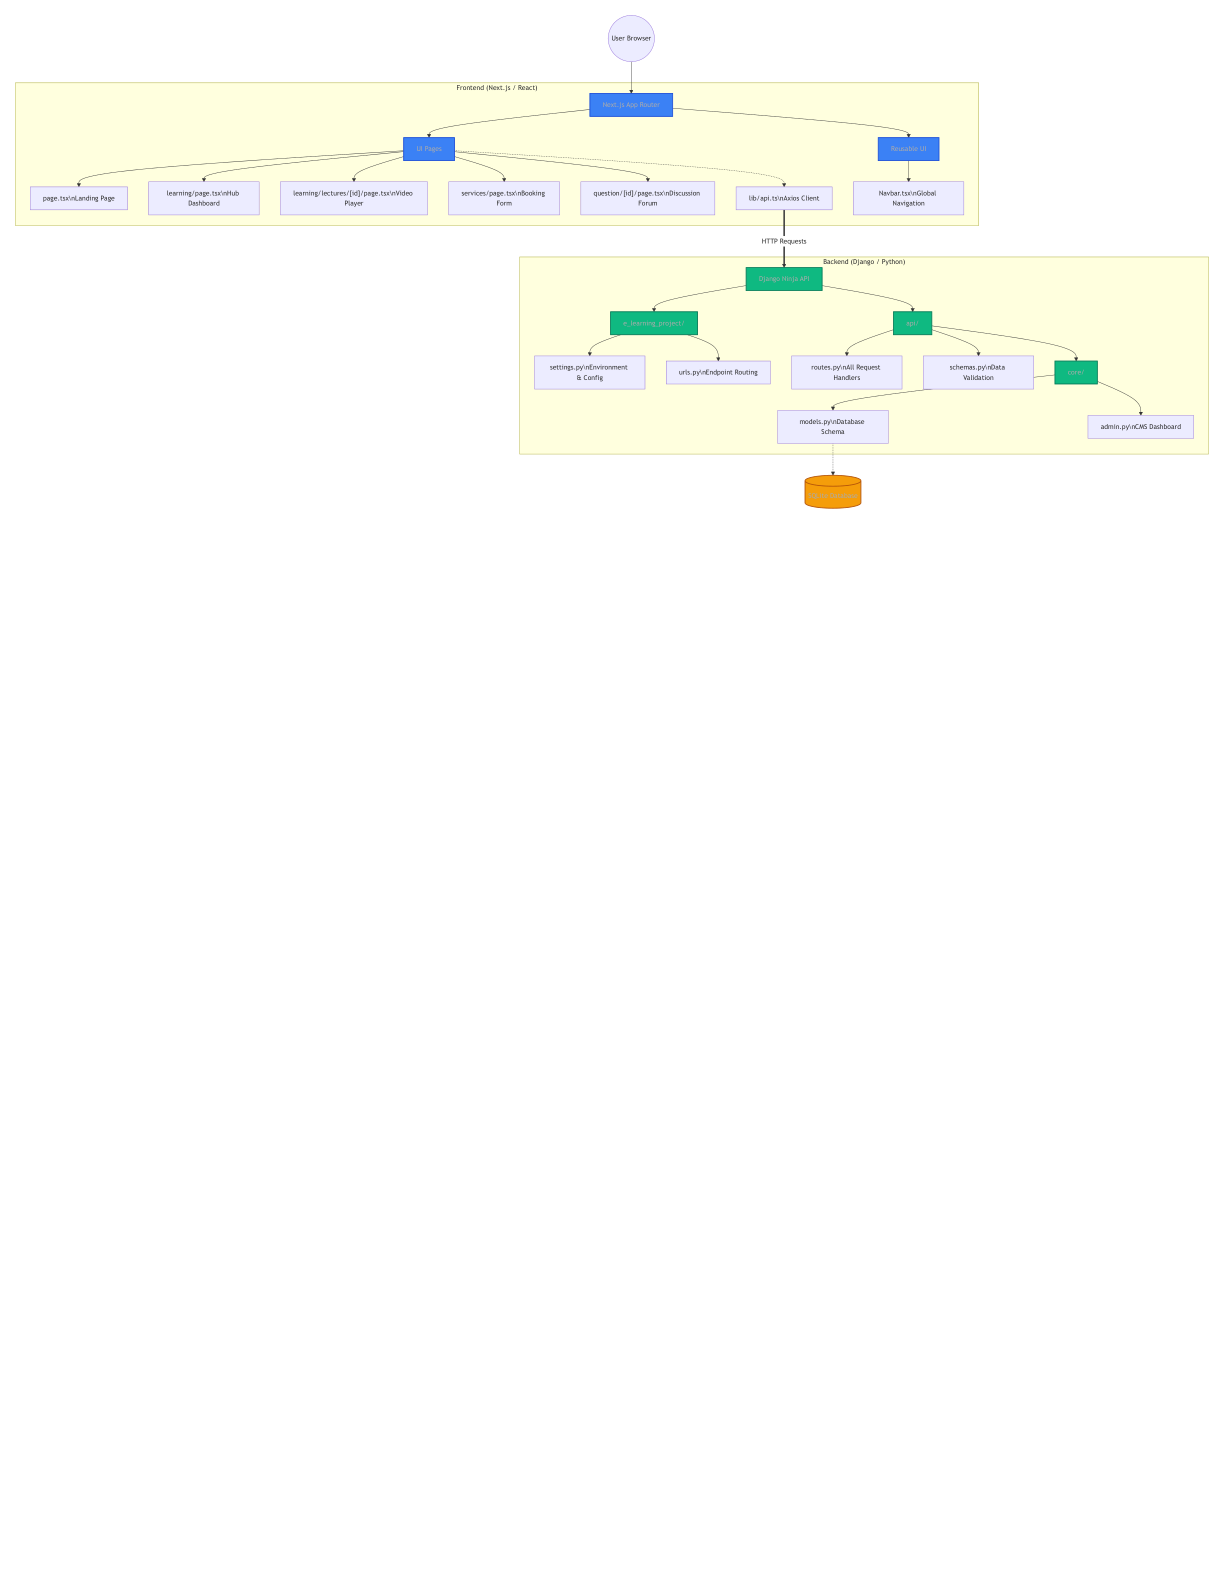
\includegraphics[width=0.9\textwidth]{neuralspark_arch.png}
    \caption{System Architecture of NeuralSpark}
    \label{fig:architecture}
\end{figure}

The three tiers are:
\begin{enumerate}
    \item \textbf{Presentation Tier:} Next.js 16 frontend served via Vercel's Edge Network.
    \item \textbf{Application Tier:} Django 6 backend with Django Ninja REST API, hosted on Render.com.
    \item \textbf{Data Tier:} SQLite (development) / PostgreSQL (production) managed by Django ORM.
\end{enumerate}

\section{Module Design}

\subsection{Learning Hub Module}
Manages video lectures organized by subject categories. The \texttt{Lecture} model links to
a \texttt{Category} via a ForeignKey and includes an \texttt{order} field for chapter sequencing.
The frontend displays lectures as a filtered, sortable grid.

\subsection{PYQ (Practice Questions) Module}
Stores previous year examination questions with their answers and optional video explanations.
Each PYQ is associated with a subject \texttt{Category} and a \texttt{year}, enabling year-wise
and subject-wise filtering on the frontend.

\subsection{Community Q\&A Module}
A Stack Overflow-inspired forum. Students post \texttt{Question} objects, attach \texttt{Tag}s,
and optionally embed video explanations. Other students submit \texttt{Answer}s which are
moderation-gated (\texttt{is\_approved}). Voting is implemented via dedicated upvote/downvote endpoints.

\subsection{AI Grader Module (Groq Cloud)}
Accepts a multipart/form-data request containing the question, rubric, and student answer
(as text and/or uploaded files). The \texttt{\_process\_uploaded\_file} helper routes PDFs
to PyPDF2 text extraction and images to base64 encoding. The compiled payload is sent to the
Groq Vision LLM (\texttt{llama-4-scout-17b-16e-instruct}), which returns a structured score
and feedback string.

\subsection{AI Grader Module (Local Transformer)}
An alternative grading pipeline using a locally hosted \texttt{AutoModelForSequenceClassification}
model. The model is lazy-loaded on first request and cached globally. It processes text-only input
and returns a numeric similarity/quality score.

\subsection{Store \& Services Module}
Products (digital goods like mock tests) and Services (mentorship sessions) are stored as
separate models. An \texttt{Inquiry} model captures service bookings from the contact form.

\section{Data Flow Diagram}

\begin{figure}[h]
    \centering
    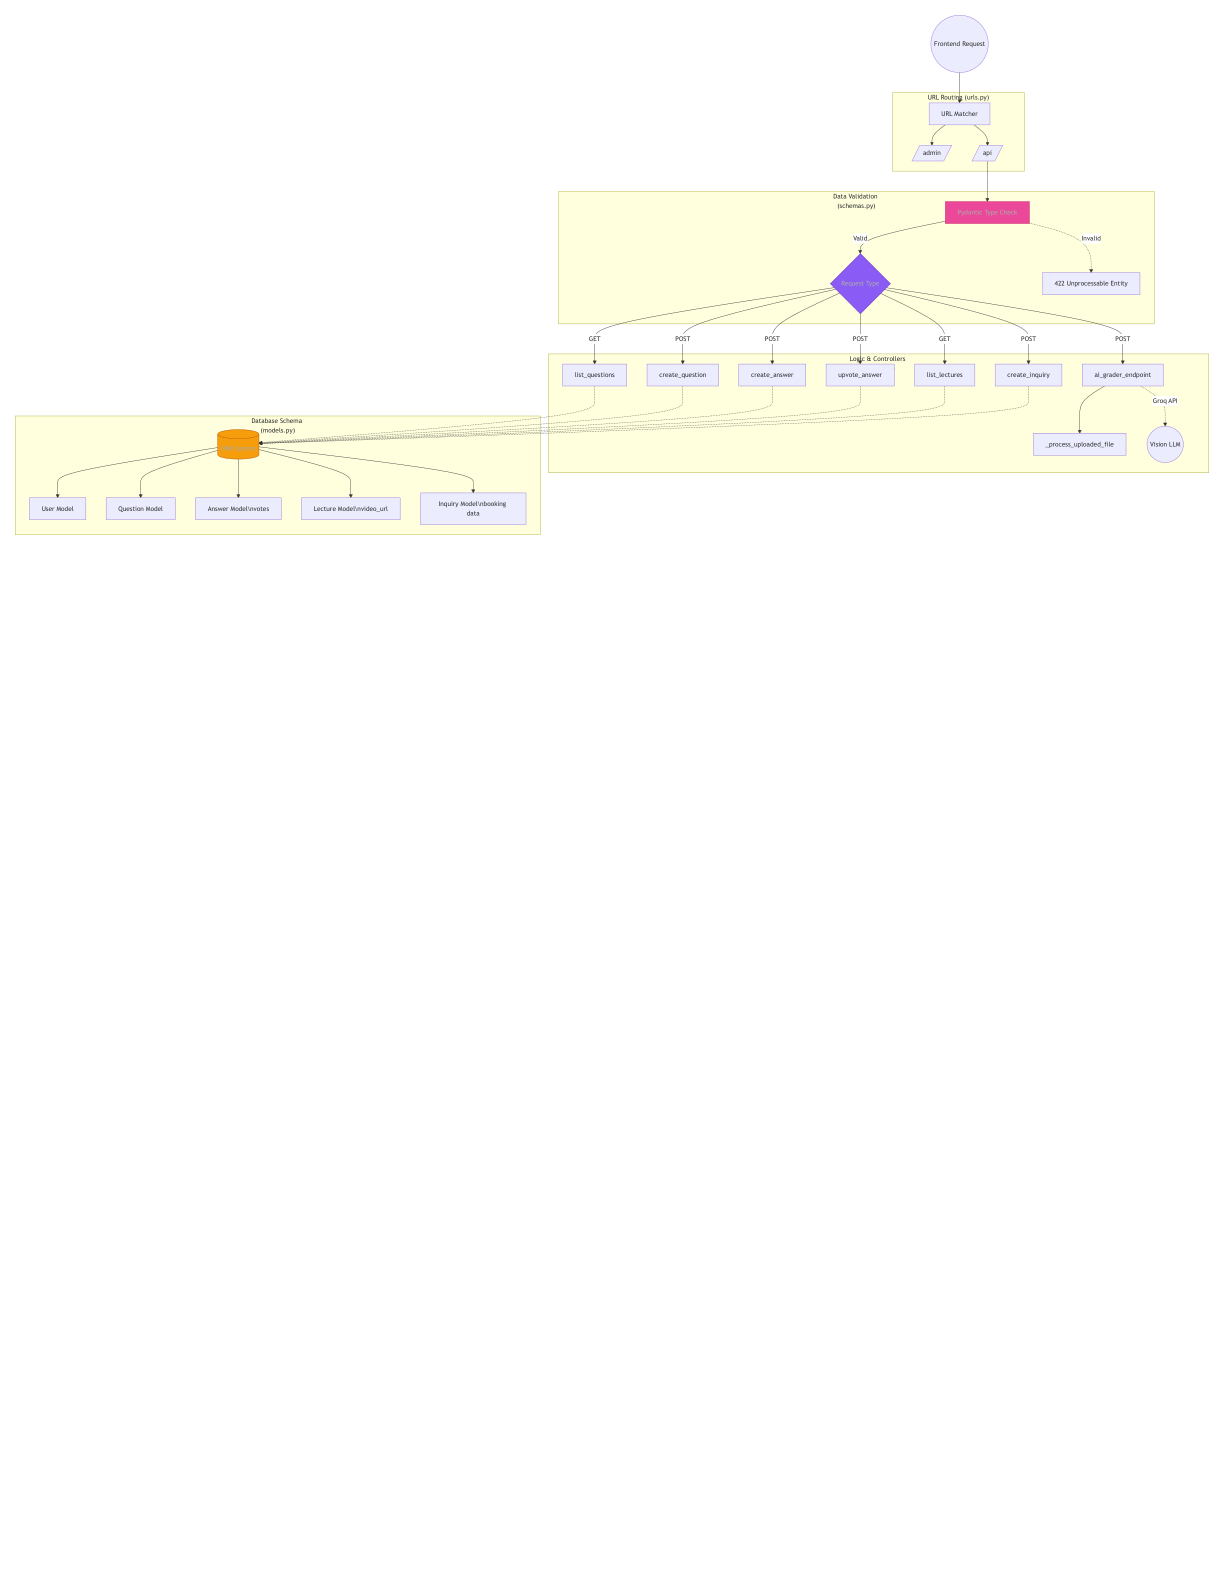
\includegraphics[width=0.9\textwidth]{neuralspark_backend_flow.png}
    \caption{Data Flow Diagram of NeuralSpark}
    \label{fig:dfd}
\end{figure}

The DFD in Figure \ref{fig:dfd} illustrates the flow of data from a student's browser request
through to the database and AI grader, and back to the client as a JSON response.

\section{Custom AI Grader Architecture}

\begin{figure}[h]
    \centering
    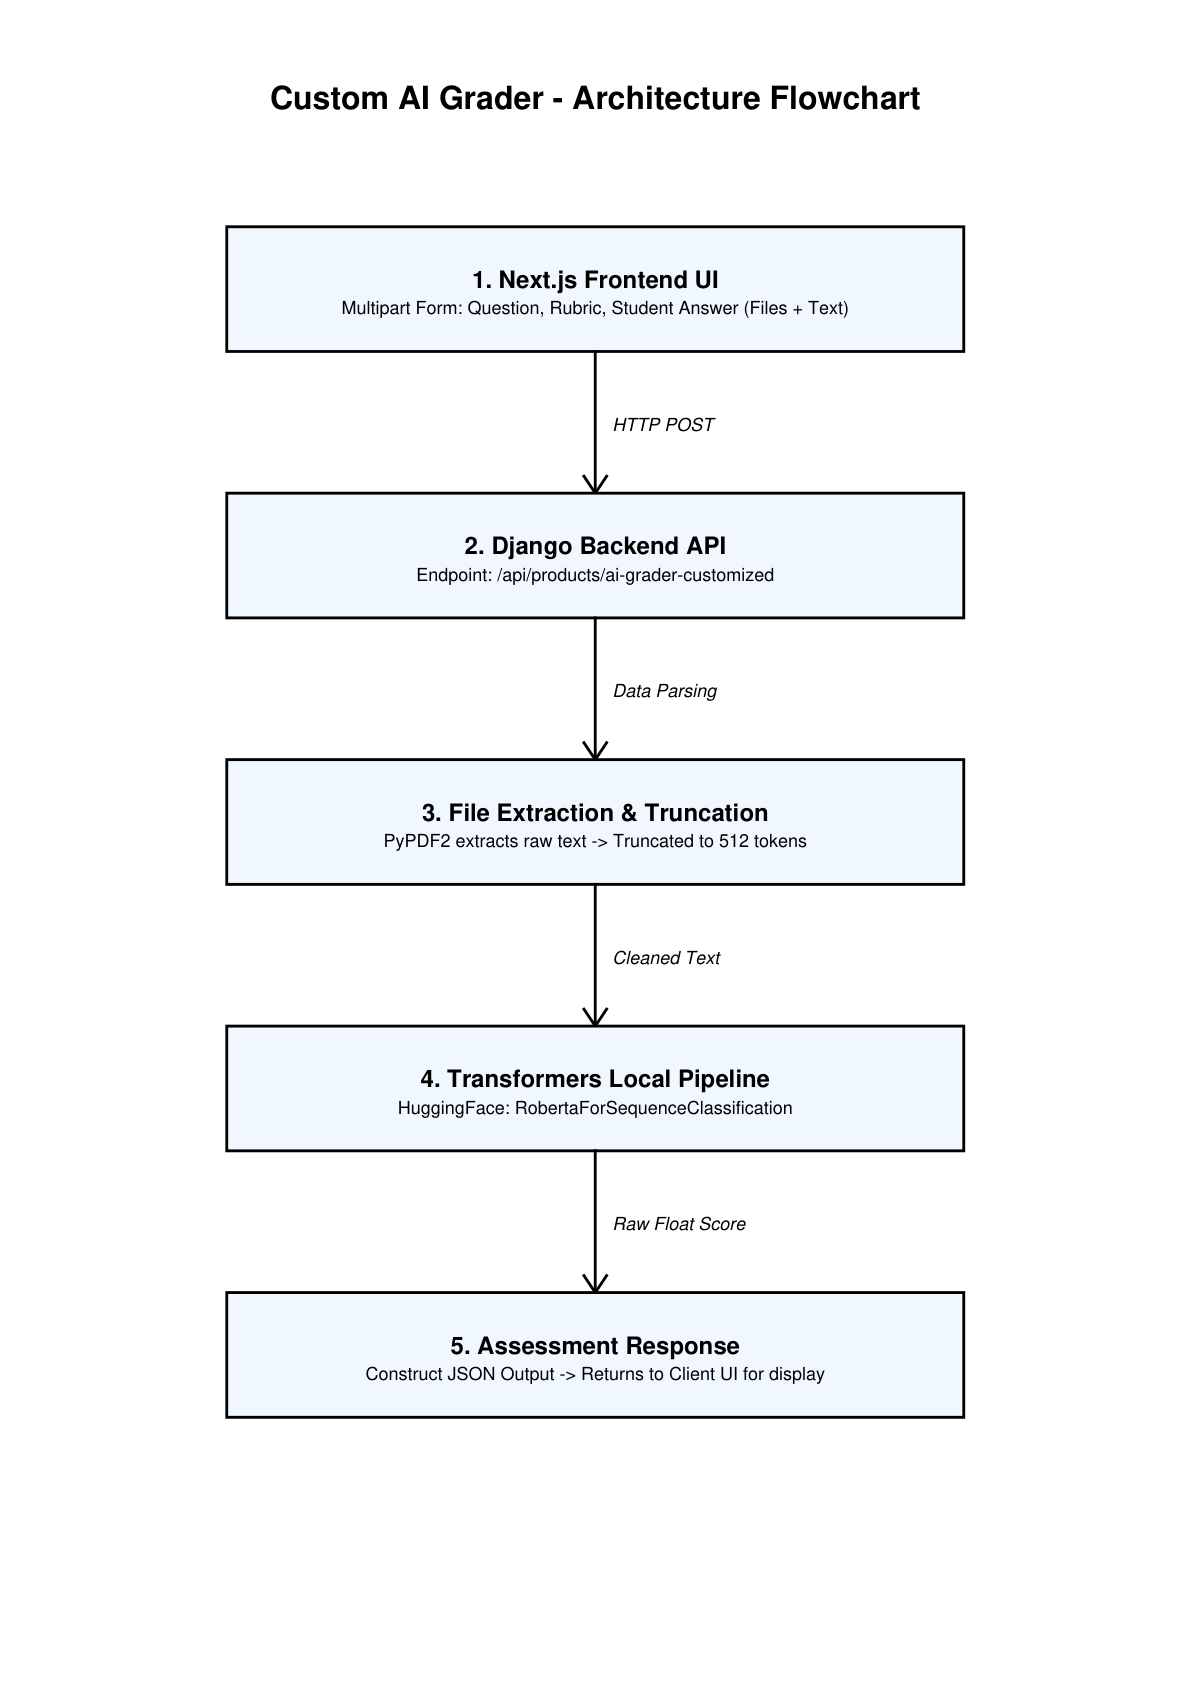
\includegraphics[width=0.85\textwidth]{custom_ai_grader_arch.png}
    \caption{Custom Local AI Grader Architecture}
    \label{fig:customai}
\end{figure}

Figure \ref{fig:customai} shows the architecture of the local AI grader, including the lazy
loading pattern, the tokenizer pipeline, and the classification head that produces the final score.

\section{Database Schema}
The relational schema consists of 11 core tables:
\texttt{User}, \texttt{Tag}, \texttt{Category}, \texttt{Lecture}, \texttt{PYQ},
\texttt{Product}, \texttt{Service}, \texttt{Question}, \texttt{Answer},
\texttt{Comment}, and \texttt{Inquiry}.

Key relationships include:
\begin{itemize}
    \item \texttt{Question} has a ManyToMany relationship with \texttt{Tag}.
    \item \texttt{Lecture} and \texttt{PYQ} have ForeignKey relationships to \texttt{Category}.
    \item \texttt{Answer} and \texttt{Comment} cascade-delete when their parent \texttt{Question} is deleted.
    \item \texttt{Inquiry} optionally links to a \texttt{Service} via a nullable ForeignKey.
\end{itemize}

\section{Design Considerations}
\begin{itemize}
    \item \textbf{Separation of Concerns:} The AI grading logic is entirely encapsulated within the API layer, not in models or views.
    \item \textbf{Lazy Loading:} The Transformer model is loaded on first use to conserve server memory.
    \item \textbf{Schema Validation:} All requests are validated by Pydantic schemas before reaching business logic.
    \item \textbf{Modular Frontend:} React components are kept small and reusable, consuming the API via Axios.
\end{itemize}

% ============================================
% CHAPTER 5: METHODOLOGY
% ============================================
\chapter{Methodology}

\section{Overview}
NeuralSpark was developed using an iterative, agile-inspired methodology. The development was
organized into functional sprints, each targeting a specific module (Forum, Learning Hub, AI Grader, etc.).

\section{Development Workflow}

\begin{table}[h]
\centering
\begin{tabular}{@{}clp{8cm}@{}}
\toprule
\textbf{Phase} & \textbf{Activity} & \textbf{Description} \\
\midrule
1 & Requirements & Defined functional and non-functional requirements \\
2 & Database Design & Designed relational schema in Django models \\
3 & API Development & Implemented all endpoints with Django Ninja \\
4 & Frontend Build & Built Next.js pages and React components \\
5 & AI Integration & Integrated Groq API and local Transformer model \\
6 & Testing & Unit tested backend; ran E2E tests via Swagger UI \\
7 & Deployment & Deployed to Vercel (frontend) and Render (backend) \\
\bottomrule
\end{tabular}
\caption{System Development Workflow}
\label{tab:workflow}
\end{table}

\section{Backend API Design}
The API was designed following RESTful conventions. Django Ninja handles routing, schema
validation, and OpenAPI documentation automatically. Each endpoint corresponds to a single
business operation (e.g., upvoting an answer, submitting a grading request).

\section{AI Grader Prompt Engineering}
The Groq grader uses a carefully engineered system prompt that instructs the model to:
\begin{enumerate}
    \item Act as an expert Computer Science teaching assistant.
    \item Strictly follow the provided rubric.
    \item Output results in a structured format: \texttt{Score: X/Y} followed by \texttt{Feedback: ...}
\end{enumerate}

The \texttt{temperature} parameter is set to \texttt{0.1} to ensure consistent, deterministic outputs.

\section{File Processing Strategy}
The \texttt{\_process\_uploaded\_file} function implements a strategy pattern:
\begin{itemize}
    \item \textbf{PDF files:} Iterated page-by-page using PyPDF2's \texttt{PdfReader}; text concatenated and returned as a text message.
    \item \textbf{Image files:} Binary content read, base64-encoded, and formatted as a \texttt{data:image/jpeg;base64,...} URI for the vision model.
\end{itemize}

\section{Local Model Inference Pipeline}
The local grader pipeline is initialized using HuggingFace's \texttt{AutoTokenizer} and
\texttt{AutoModelForSequenceClassification.from\_pretrained()}. The model is loaded from a local
directory (\texttt{ai\_grader\_model\_customized/}) to avoid internet dependency at inference time.
Inputs are truncated to a maximum of 512 tokens to prevent out-of-memory errors.

\section{Frontend Rendering Strategy}
The frontend uses a hybrid rendering approach:
\begin{itemize}
    \item \textbf{Server Components:} Used for static content and page layouts.
    \item \textbf{Client Components:} Used for interactive elements (\texttt{"use client"} directive) including the AI Grader form and the dark mode toggle.
\end{itemize}

\section{Theme Management}
The \texttt{ThemeContext} provides a global dark/light mode toggle. The theme is persisted to
\texttt{localStorage} on every toggle, and the system preference (\texttt{prefers-color-scheme})
is read on initial load via a \texttt{useEffect} hook.

\section{Summary}
The methodology followed a clean separation of concerns at every layer: schema-first API design,
component-first frontend development, and strategy-pattern file processing for the AI grader.
This structured approach ensured each module remained independently testable and replaceable.

% ============================================
% CHAPTER 6: IMPLEMENTATION
% ============================================
\chapter{Implementation}

\section{Introduction}
This chapter details the technical implementation of NeuralSpark, covering the development
environment, module implementations, system integration, and output.

\section{Development Environment}

\begin{table}[h]
\centering
\begin{tabular}{@{}ll@{}}
\toprule
\textbf{Tool} & \textbf{Details} \\
\midrule
OS & Windows 11 \\
IDE & Visual Studio Code \\
Version Control & Git + GitHub \\
Python Version & 3.12 \\
Node.js Version & 22.x (LTS) \\
Package Manager & pip (backend), npm (frontend) \\
Deployment & Vercel (frontend), Render.com (backend) \\
\bottomrule
\end{tabular}
\caption{Development Environment}
\label{tab:devenv}
\end{table}

\section{System Implementation}

\subsection{Backend Initialization}
The backend was initialized using \texttt{django-admin startproject} and configured with a custom
\texttt{User} model extending \texttt{AbstractUser}. Django Ninja's \texttt{NinjaAPI} instance
is mounted at \texttt{/api/} in the project's URL configuration.

\subsection{Database Models}
All eleven database models (\texttt{User}, \texttt{Tag}, \texttt{Category}, \texttt{Lecture},
\texttt{PYQ}, \texttt{Product}, \texttt{Service}, \texttt{Question}, \texttt{Answer},
\texttt{Comment}, \texttt{Inquiry}) were defined in \texttt{backend/core/models.py} and
registered via Django Admin for content management.

\subsection{API Endpoints}
Seventeen REST API endpoints were implemented in \texttt{backend/api/routes.py}:

\begin{table}[h!]
\centering
\begin{tabular}{@{}p{6cm}p{1.5cm}p{5cm}@{}}
\toprule
\textbf{Endpoint} & \textbf{Method} & \textbf{Description} \\
\midrule
\texttt{/api/hello/} & GET & API health check \\
\texttt{/api/questions/} & GET & List all forum questions \\
\texttt{/api/questions/} & POST & Create a new question \\
\texttt{/api/questions/\{id\}/} & GET & Get question + increment views \\
\texttt{/api/questions/\{id\}/answers/} & GET & Get approved answers \\
\texttt{/api/questions/\{id\}/answers/} & POST & Submit an answer \\
\texttt{/api/answers/\{id\}/upvote/} & POST & Upvote an answer \\
\texttt{/api/answers/\{id\}/downvote/} & POST & Downvote an answer \\
\texttt{/api/answers/\{id\}/comments/} & POST & Comment on an answer \\
\texttt{/api/categories/} & GET & List all subject categories \\
\texttt{/api/lectures/} & GET & List ordered video lectures \\
\texttt{/api/pyqs/} & GET & List PYQs by year \\
\texttt{/api/products/} & GET & List all products \\
\texttt{/api/services/} & GET & List all services \\
\texttt{/api/inquiries/} & POST & Submit a service inquiry \\
\texttt{/api/products/ai-grader/} & POST & Grade with Groq Cloud LLM \\
\texttt{/api/products/ai-grader-customized/} & POST & Grade with local Transformer \\
\bottomrule
\end{tabular}
\caption{NeuralSpark API Endpoints}
\label{tab:endpoints}
\end{table}

\subsection{AI Grader Implementation}
The Groq AI Grader accepts a \texttt{multipart/form-data} request with up to three text fields
and three file fields. The \texttt{\_process\_uploaded\_file} function dispatches each file
to the appropriate processor (PDF → text, image → base64 URI). The compiled message list is
sent to the Groq API in a single \texttt{chat.completions.create} call.

The local grader uses \texttt{get\_custom\_grader\_pipeline()}, a thread-safe lazy loader
that initializes the HuggingFace pipeline once per server lifetime.

\subsection{Frontend Implementation}
The frontend consists of multiple Next.js App Router pages:
\begin{itemize}
    \item \texttt{/} (Landing Page): Hero section with Framer Motion stagger animations.
    \item \texttt{/learning} (Lectures): Grid of video lecture cards, filterable by category.
    \item \texttt{/learning/pyqs} (PYQs): Accordion list of previous year questions.
    \item \texttt{/learning/questions} (Forum): Community Q\&A board with voting.
    \item \texttt{/products} (Store): Product cards with external purchase links.
    \item \texttt{/products/ai-grader} (AI Grader): Multimodal grading form.
    \item \texttt{/services} (Services): Service listings with inquiry form.
\end{itemize}

\subsection{Deployment}
The backend was deployed to Render.com by configuring \texttt{gunicorn} as the WSGI server
and \texttt{whitenoise} for static file serving. \texttt{ALLOWED\_HOSTS} and \texttt{CORS\_ALLOW\_ALL\_ORIGINS}
were configured for the production domain. The frontend was deployed to Vercel by connecting
the GitHub repository, with \texttt{NEXT\_PUBLIC\_API\_URL} set as an environment variable.

\section{System Integration and Testing}
The system was integration-tested using Django Ninja's auto-generated Swagger UI at
\texttt{/api/docs}. Each endpoint was tested with representative payloads. The AI Grader
was tested with a sample rubric and student answer, validating the structured output format.

\section{System Output}
\begin{figure}[h]
    \centering
    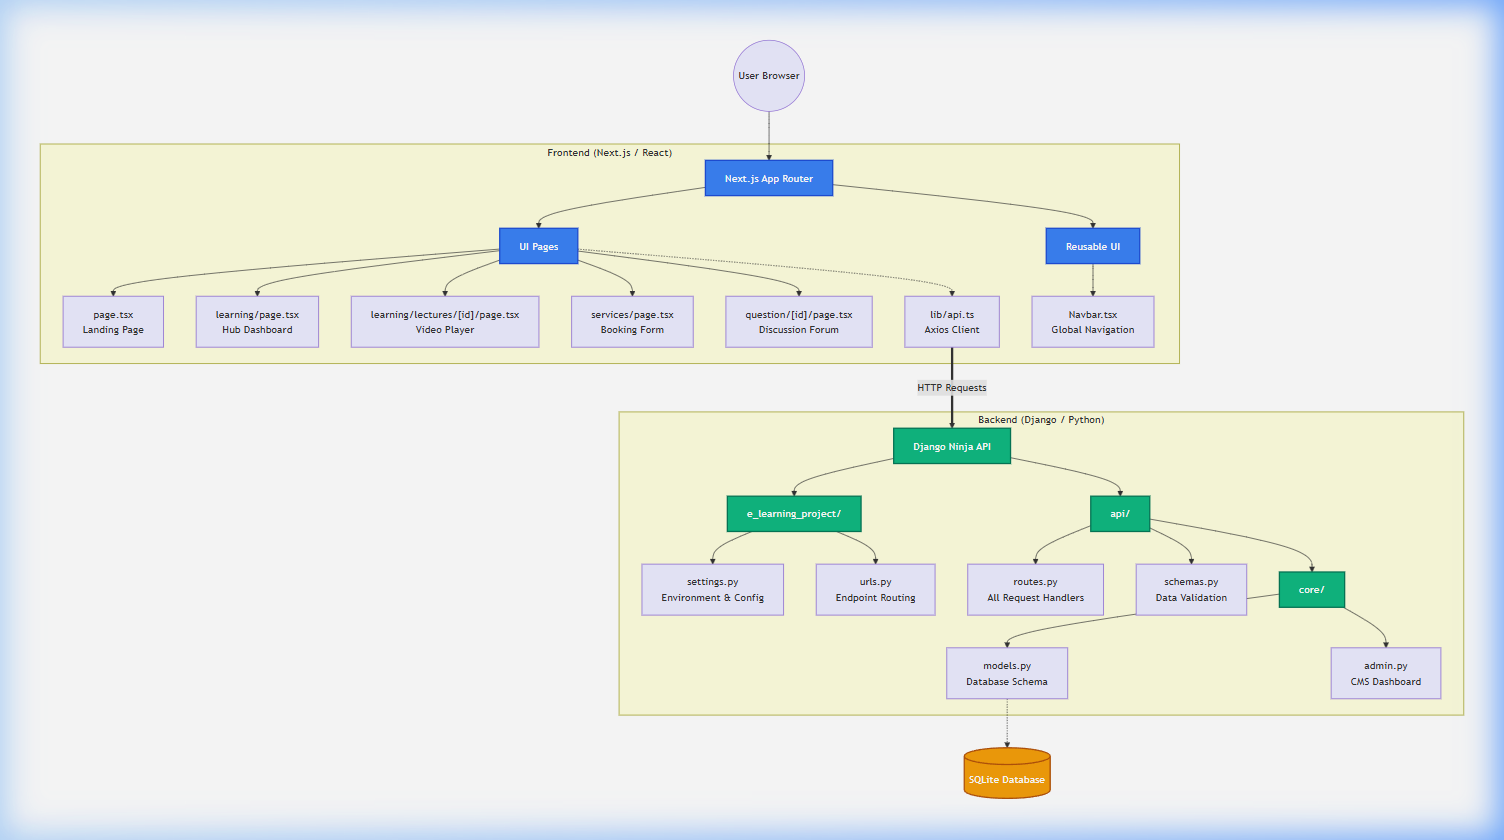
\includegraphics[width=0.9\textwidth]{arch_diagram.png}
    \caption{NeuralSpark Component Architecture Diagram}
    \label{fig:output1}
\end{figure}

\begin{figure}[h]
    \centering
    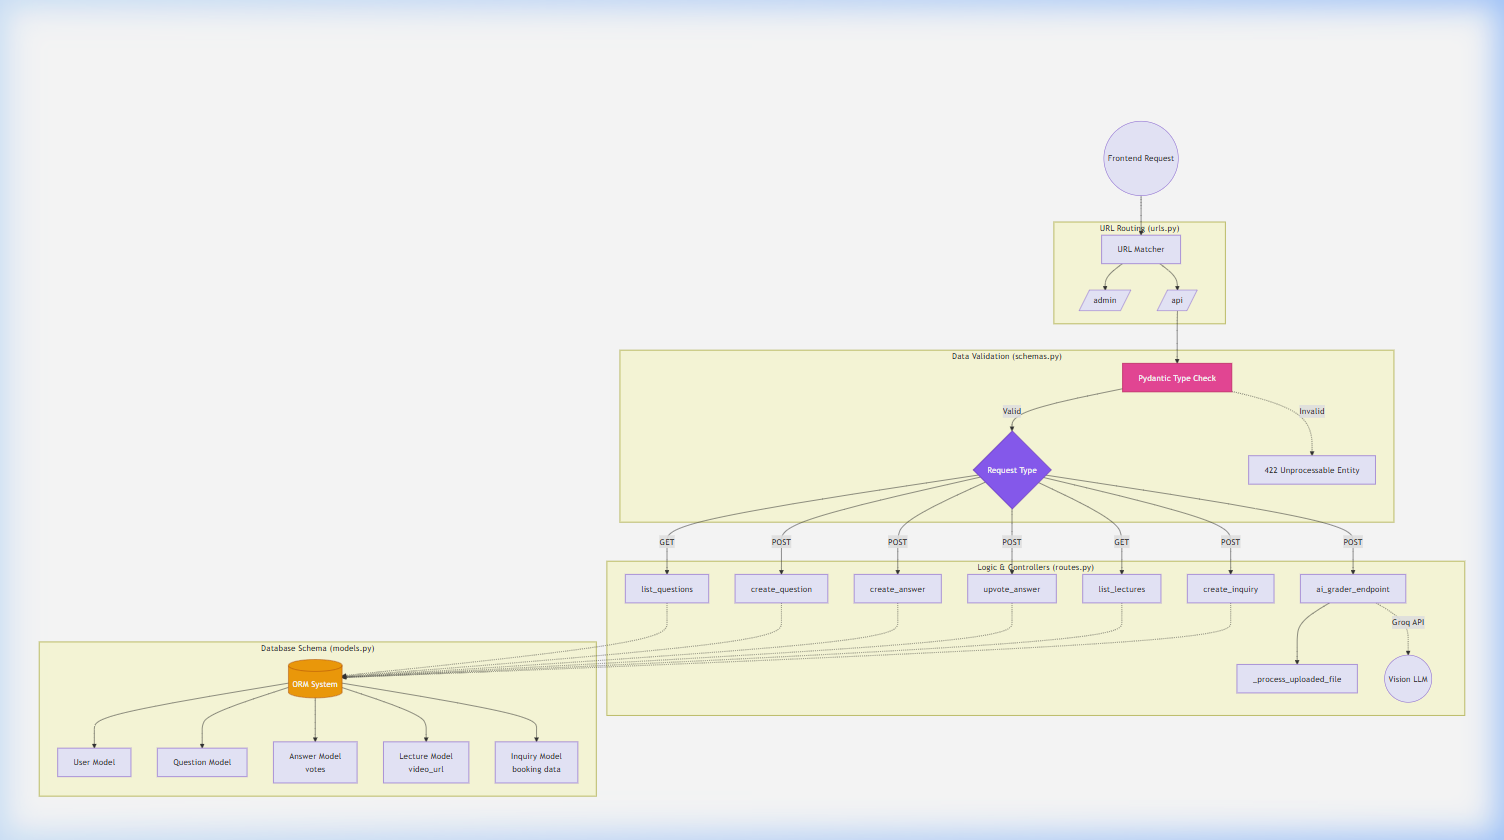
\includegraphics[width=0.9\textwidth]{flow_diagram.png}
    \caption{NeuralSpark Backend Data Flow Diagram}
    \label{fig:output2}
\end{figure}

\section{Summary}
The implementation of NeuralSpark successfully delivered all seven core modules. The AI Grader
endpoint correctly processes text, PDF, and image inputs and returns structured scores and
feedback. The frontend achieves a premium aesthetic through Tailwind CSS and Framer Motion animations.

% ============================================
% CHAPTER 7: CONCLUSION
% ============================================
\chapter{Conclusion}

NeuralSpark demonstrates that a production-quality, AI-integrated e-learning platform can be
built by a single developer using modern, open-source technologies. The project successfully
addresses the core problem of automated, fair, and multimodal assignment grading through two
complementary pipelines: the Groq Cloud Vision LLM for high-accuracy grading and a locally
hosted Transformer model for privacy-first and offline environments.

The Community Q\&A Forum, Learning Hub, and PYQ Repository provide a holistic educational
ecosystem beyond just grading. The platform's clean decoupled architecture — with a Django
Ninja REST API and a standalone Next.js frontend — ensures that each component is independently
maintainable and scalable.

All stated objectives of the project have been met:
\begin{itemize}
    \item A functional full-stack web application built with Django 6 + Next.js 16.
    \item A multimodal AI grader supporting text, PDF, and image inputs.
    \item Two independent grading pipelines (cloud and local).
    \item A complete community forum with voting and moderation.
    \item A learning module with video lectures and PYQ banks.
    \item Successful deployment on Vercel and Render.com.
\end{itemize}

% ============================================
% CHAPTER 8: FUTURE WORK
% ============================================
\chapter{Future Work}

\section{Real-Time Collaboration}
Implementing Django Channels (WebSockets) would enable real-time collaborative learning sessions,
live doubt-solving, and real-time peer code review within the forum.

\section{Advanced Authentication}
Replacing the current test-user placeholder with a full JWT-based authentication system
(using \texttt{djangorestframework-simplejwt}) would enable personalized dashboards,
submission history, and reputation-based access controls.

\section{Mobile Application}
A React Native mobile application sharing the same Django Ninja backend would extend
NeuralSpark's reach to mobile learners, enabling offline access to PYQs and lecture notes.

\section{Fine-Tuned Rubric-Aware Model}
The local Transformer model can be further fine-tuned on a domain-specific dataset of
Computer Science assignment submissions and expert grades to improve its accuracy beyond
general-purpose text classification.

\section{Multi-Language Support}
Adding i18n support to the frontend and extending the AI grader to support non-English
rubrics (e.g., Hindi, Tamil) would make the platform accessible to a broader student population.

\section{Analytics Dashboard}
An instructor-facing analytics dashboard showing submission trends, average scores,
common mistakes, and student performance over time would add significant educational value.

% ============================================
% BIBLIOGRAPHY
% ============================================
\begin{thebibliography}{99}

\bibitem{devlin2019bert}
J. Devlin, M.-W. Chang, K. Lee, and K. Toutanova, ``BERT: Pre-training of Deep Bidirectional Transformers for Language Understanding,'' \textit{arXiv preprint arXiv:1810.04805}, 2019.

\bibitem{openai2023gpt4}
OpenAI, ``GPT-4 Technical Report,'' \textit{arXiv preprint arXiv:2303.08774}, 2023.

\bibitem{wang2022multimodal}
X. Wang et al., ``Multimodal Assessment Frameworks for E-Learning,'' \textit{IEEE Transactions on Learning Technologies}, vol. 15, no. 3, 2022.

\bibitem{porchet2023djangoninja}
M. Porchet, ``Comparative Analysis of Python REST API Frameworks,'' \textit{Software Engineering Journal}, 2023.

\bibitem{vercel2023rsc}
Vercel Engineering, ``Understanding React Server Components,'' \textit{Vercel Blog}, 2023. [Online]. Available: \url{https://vercel.com/blog/understanding-react-server-components}

\bibitem{groq2024api}
Groq Inc., ``Groq API Documentation,'' 2024. [Online]. Available: \url{https://console.groq.com/docs}

\bibitem{huggingface2023transformers}
HuggingFace, ``Transformers Library Documentation,'' 2023. [Online]. Available: \url{https://huggingface.co/docs/transformers}

\bibitem{django2024docs}
Django Software Foundation, ``Django 6.0 Documentation,'' 2024. [Online]. Available: \url{https://docs.djangoproject.com}

\bibitem{vienot2023fpdf2}
O. Vienot, ``fpdf2: FPDF for Python,'' 2023. [Online]. Available: \url{https://py-pdf.github.io/fpdf2/}

\bibitem{pypdf2023}
PyPDF2 Contributors, ``PyPDF2 Documentation,'' 2023. [Online]. Available: \url{https://pypdf2.readthedocs.io}

\end{thebibliography}

\end{document}
